\chapter{Theoretical Overview}
The primary resources used in the writing of the chapter were \cite{mann,griffiths,sood}. These should be consulted for further reading.
\section{The Standard Model of Particle Physics}
The Standard Model \cite{SM1,SM2,SM3,SM4} of particle physics was developed in the latter half of the twentieth century. It describes how matter is comprised of point-like, basic building blocks, called fundamental particles, which interact via three fundamental forces. The Standard Model has been tested successfully many times and is widely regarded as the most accurate and stable \cite{SM_fit} model of particle physics. It classifies the fundamental particles that make up matter into either leptons or quarks. Both leptons and quarks come in three so-called generations, with the members of the later generations being heavier and less stable than their previous generation counterparts.\footnote{An important caveat to this are the neutrinos, which do not decay, and whose tiny non-zero mass is not known to be related to their generation.} In ascending order of generation, the leptons are: the electron and electron neutrino, the muon and muon neutrino, and the tau and tau neutrino. Quarks are also classified into three generations, with each generation having two flavours of quarks. In ascending order of generation, the quarks are: the up and down, the charm and strange, and the top and bottom. Quarks are never observed in isolation due to colour confinement and instead are only observable in bound states called hadrons. Bound states consisting of a quark-antiquark pair are called mesons, while bound states of three quarks are called baryons. Both leptons and quarks have half-integer spin.\footnote{In this thesis, spin will always be implicitly measured in units of Planck's reduced constant $\hbar$.} Particles possessing half-integer spin are known collectively as \emph{fermions}. Fermions as a collective are constrained by the Pauli exclusion principle, meaning that no two fermions may occupy the same quantum state.

The Standard Model describes three of the four fundamental interactions in nature. In increasing order of strength, these are: the weak, electromagnetic, and strong forces. According to the Standard Model: the strong, weak, and electromagnetic forces result from the exchange of force-carrier particles. These force carriers possess integer-spins  and are collectively called \emph{bosons}. Specific bosons are said to mediate a particular force. The strong force is mediated by the gluon, the electromagnetic by the photon, and the weak by the W and Z bosons. The masses of the elementary particles arise from their coupling to the Higgs field, which is mediated by the Higgs boson.

The process via which fundamental particles couple to the Higgs field and hence become massive is called the \emph{Higgs mechanism}. The Higgs boson was experimentally observed by the ATLAS and CMS collaborations in 2012 \cite{ATLAS_higgs,CMS_higgs}. At extremely hot temperatures\footnote{When the equilibrium thermal energy of the system is on the order of 100 GeV.} the W and Z bosons are effectively massless and the electromagnetic and weak forces become practically indistinguishable. They are, in fact, different aspects of the same unified electroweak force or \emph{electroweak interaction}. Below the aforementioned sufficiently high temperature, this symmetry is spontaneously broken, resulting in the W and Z bosons having mass via the Higgs mechanism and making the electromagnetic and weak forces appear distinct. This is discussed in more detail in the following section \ref{ewk uni}. Both the strong and electroweak interactions are described by their corresponding \emph{gauge theories}\footnote{The reader may find useful a brief review of gauge theories provided in appendix \ref{appendix1}.}, with \emph{Quantum ChromoDynamics} (QCD) describing the former and \emph{electroweak field theory} describing the latter.

A deficiency of the Standard Model is that it does not describe the gravitational interaction. Theories that seek to expand upon the Standard Model in order to, for example, incorporate gravity are said to be ``beyond'' the Standard Model.
\begin{figure}
\centering
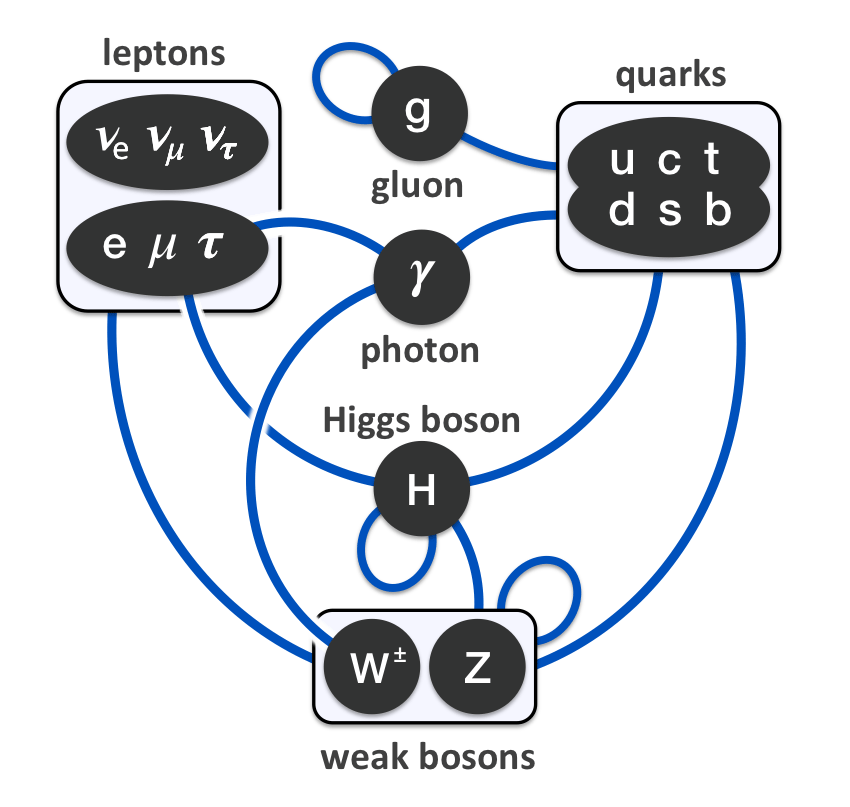
\includegraphics[width=0.55\textwidth]{images/fund_part_in_sm.png}
\label{sm_part_image}
\caption{Illustration of the fundamental particles described by the Standard Model, showing how they interact amongst each other and sometimes themselves. \cite{fund_part_image}}
\end{figure}
\section{Electroweak Unification}
\label{ewk uni}
As previously mentioned the electromagnetic and weak interactions are actually different manifestations of the same electroweak interaction. This is reflected in the \emph{electroweak unification} model; primarily developed by Glashow, Salam, and Weinberg in the 1960s. In 1971 't Hooft and Veltmann showed that the model is renormalisable\footnote{A renormalisable gauge theory is one in which any infinities introduced by the inclusion of higher-order diagrams can be absorbed by modification of a finite number of parameters. All the gauge theories of the Standard Model are renormalisable. In contrast General Relativity isn't renormalisable, leading to problems for theories attempting to include Quantum Gravity.} \cite{renorm1,renorm2,renorm3,renorm4} which has been confirmed by many subsequent particle physics experiments \cite{SM_fit}. The full electroweak theory has a non-abelian symmetry $\mathbf{SU}(2) \otimes \mathbf{U}(1)$; with three gauge bosons $ \left\{ W_{\mu}^{1},W_{\mu}^{2},W_{\mu}^{3} \right\} = \mathbf{W}_{\mu}$ being associated with $\mathbf{SU}(2)$ and one gauge boson $B_{\mu}$ being associated with $\mathbf{U}(1)$. The physical interpretation of the fact that the symmetry is non-abelian is that the $W_{\mu}$ and $B_{\mu}$ bosons interact amongst themselves and with each other.

However the symmetry is broken. The mixing of the wavefunctions for the $W_{\mu}^{3}$ and $B_{\mu}$  results in the neutral Z-boson and the photon; while the remaining $W_{\mu}^{1}$ and $W_{\mu}^{2}$ result in the charged $W^{\pm}$ bosons. The reason why the wavefunctions mix to form the neutral bosons, and why the photons is massless while the W and Z bosons are not, is understood in the context of \emph{spontaneous symmetry breaking} and the Higgs mechanism.
\section{Electroweak Symmetry Breaking}
\label{Higgs_section}
In the SM, the electroweak symmetry is spontaneously broken resulting in masses for the weak bosons and fermions via the Higgs mechanism.

To demonstrate this consider a complex scalar field $\phi$, representing the Higgs field. It is taken to have hypercharge\footnote{Hypercharge $Y$ is a number related to electric charge Q via the Gell-Mann-Nishijima formula: $ Y = 2(Q - T_{3})$, where $T_{3}$ is the third component of weak isospin ($ \pm 1/2$ for left-handed fermion and $0$ for right-handed fermions).} $Y = +1$, weak isospin $1/2$, and transforms as a doublet\footnote{\emph{Multiplet} is a common name for a wavefunction with multiple components. So a doublet has two components, a triplet has three, etc.} under $\mathbf{SU}(2)$.

In analogy with classical mechanics, the Lagrangian is consider in kinetic and potential parts:
\begin{eqnarray}
T &=& \left( D_{\mu} \phi \right) ^{\dagger} D^{\mu} \phi \\
V &=& -\mu^{2} | \phi | ^{2} + \lambda | \phi | ^{4},
\end{eqnarray}
where $D_{\mu}$ is the covariant derivative defined as:
\begin{equation}
D_{\mu} \equiv \partial_{\mu} - ig \frac{\sigma ^{a}}{2} W_{\mu}^{a} - i \frac{g'}{2}B_{\mu},
\end{equation}
$\mu ^{2}$ and $\lambda$ are real constants, $\sigma^{a}$ are the Pauli spin matrices, $g$ is the weak coupling and $g'$ the hypercharge coupling (both dimensionless), and the latin indices run $a = (1,2,3)$.

Assuming $\mu^{2}$ and $\lambda$ are positive implies that the ground state of the system (it's vacuum) will have a non-zero \emph{vacuum expectation value} (VEV). The potential $V$ is solely a function of the magnitude of $\phi$ and takes the form of the (famous) Mexican hat potential (see figure \ref{mexican_hat}). This means that there is no inherent single vacuum (ground state). Defining:
\begin{equation}
v = \sqrt{\mu^{2}/\lambda},
\end{equation}
the VEV can be chosen to be:
\begin{eqnarray}
\left< \phi \right> = \frac{1}{\sqrt{2}}
	\begin{pmatrix}
	0 \\
	v
	\end{pmatrix}.
\end{eqnarray}
The choice of vacuum breaks the electroweak symmetry. It is called \emph{spontaneous} because it occurs without any external interference. Left to its own devices, the system will tend to an inherently asymmetrical vacuum. Note that while the $\mathbf{SU}(2)$ symmetry is broken, the $\mathbf{U}(1)$ symmetry of the electromagnetic interaction remains intact.
\begin{figure}
\centering
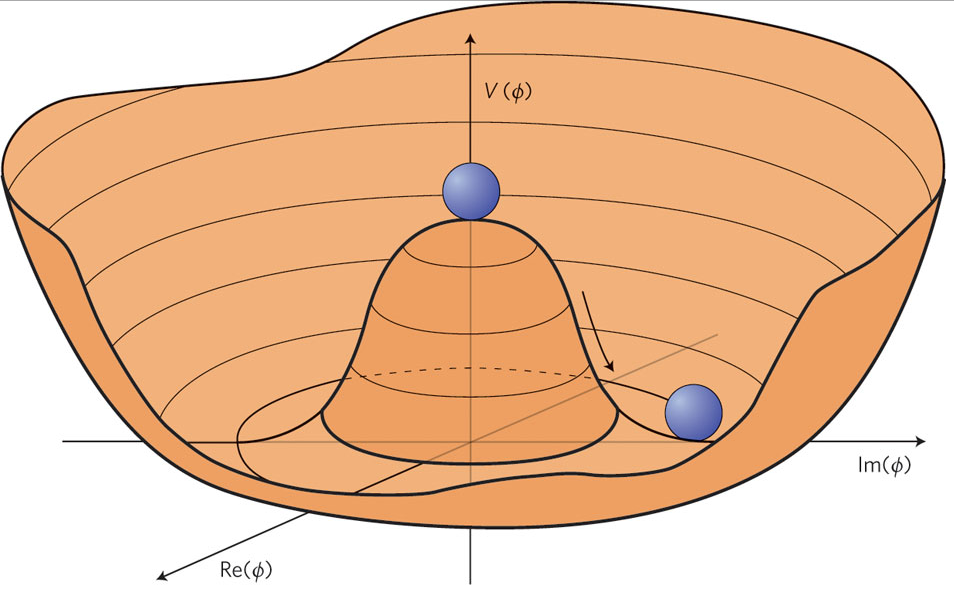
\includegraphics[width=0.65\textwidth]{images/higgs_potential.png}
\caption{Illustration of the Higgs potential. Note that it has a local maximum at the origin and a continuous ring of minima. \cite{mexican_hat}}
\label{mexican_hat}
\end{figure}
This VEV can be inserted into the kinetic term of the Lagrangian. In order to identify the mass terms, compare with the Klein-Gordon Lagrangian:
\begin{equation}
\mathcal{L} = \frac{1}{2} \left( \partial_{\mu} \phi \right) \left( \partial^{\mu} \phi \right) - \frac{1}{2}m^{2}\phi^{2}.
\end{equation}
$m^{2}$ can thus be identified as the coefficient of the quadratic field variable term. The mass terms from the kinetic Lagrangian are then:
\begin{eqnarray}
\Delta T &=& \left< \phi \right> \left( ig \frac{\sigma^{a}}{2}W_{\mu}^{a} + i \frac{g'}{2}B_{\mu} \right) \left(-ig\frac{\sigma^{b}}{2}W_{\mu}^{b} - i\frac{g'}{2}B_{\mu} \right) \left< \phi \right> \\
             &=& \frac{v^{2}}{2}\left( \frac{g^{2}}{4}W_{\mu}^{a}W^{\mu a} + \frac{{g'}^{2}}{4} B_{\mu}B^{\mu} + \frac{gg'}{2} W_{\mu}^{3}B^{\mu} \right).
             \label{mass terms}
\end{eqnarray}
Hence, a mass matrix can be constructed:
\begin{eqnarray}
m^{2} = \frac{v^{2}}{4}
	\begin{pmatrix}
	g^{2} & 0 & 0 & 0 \\
	0 & g^{2} & 0 & 0 \\
	0 & 0 & g^{2} & gg' \\
	0 & 0 & gg' & {g'}^{2}
	\end{pmatrix},
\end{eqnarray}
such that:
\begin{eqnarray}
m^{2} \times
	\begin{pmatrix}
	W_{\mu}^{1} \\
	W_{\mu}^{2} \\
	W_{\mu}^{3} \\
	B_{\mu}
	\end{pmatrix}
\end{eqnarray}
reproduces equation \ref{mass  terms}. The mass matrix can be diagonalised by a suitable choice of basis. Since any basis that diagonalises a matrix is the set of eigenvectors, the corresponding eigenvalues are strung across the (now diagonalised) matrix's diagonal. The canonical choice of eigenvectors and their corresponding eigenvalues are:
\begin{eqnarray}
W_{\mu}^{\pm} = \frac{1}{\sqrt{2}} \left( W_{\mu}^{1} \mp iW_{\mu}^{3} \right), \ m_{W} = \frac{g v}{2} \nonumber \\
Z_{\mu} = \frac{1}{\sqrt{g^{2} + {g'}^{2}}} \left( g'W_{\mu}^{3} - g' B_{\mu} \right), \ m_{Z} = \frac{v}{2}\sqrt{g^{2} + {g'}^{2}} \nonumber \\
A_{\mu} = \frac{1}{\sqrt{g^{2} + {g'}^{2}}} \left( g' W_{\mu}^{3} + g B_{\mu} \right), \ m_{A} = 0.
\end{eqnarray}
The mass eigenvectors are interpreted as the gauge fields for the charged weak, neutral weak, and electromagnetic interactions respectively; with the eigenvalues being the masses of their associated gauge bosons. Due to spontaneously broken $\mathbf{SU}(2)$ theorem symmetry, the W and Z bosons have acquired mass but, as the $\mathbf{U}(1)$ symmetry remains intact, the photon remains massless. This is the \emph{Higgs mechanism}; responsible for giving mass to the W and Z bosons.\footnote{The Higgs mechanism is also responsible for giving mass to fermions, though it is not shown here.}

The \emph{Feynman Calculus} is formulated in terms of deviations from the vacuum. With this in mind one can perturb the Higgs potential by four scalar fields: $w^{1}(x),w^{2}(x),w^{3}(x),$ and $h(x)$. These fields are fluctuations about the vacuum. The perturbed Higgs potential is:
\begin{eqnarray}
\phi =
	\begin{pmatrix}
	w^{1}(x) + iw^{2}(x) \\
	v + h(x) + iw^{3}(x)
	\end{pmatrix}.
\end{eqnarray}
Inserting the perturbed Higgs potential into the potential term of the Lagrangian yields:
\begin{eqnarray}
\Delta V_{perturbation} &=& \frac{-\mu^{2}}{2} \left[ \left( v + h \right)^{2} + w^{a}w^{a} \right] + \frac{\lambda}{4} \left[ \left( v + h \right)^{2} + w^{a}w^{a} \right]^{2} \nonumber \\
&=& \left( \lambda v^{3} - \mu^{2} v \right)h + \frac{1}{2} \left( 3 \lambda v^{2} - \mu^{2} \right)h^{2} + \frac{1}{2} \left( \lambda v^{2} - \mu^{2} \right) w^{a} w^{a} \nonumber \\
&+& \lambda v \left( h^{3} + hw^{a}w^{a} \right) + \frac{\lambda}{4} \left( h^{4} +2h^{2} w^{a} w^{a} \right) \nonumber \\
&=& \frac{1}{2} \left( 2 \lambda v^{2} \right) h^{2} + \lambda v \left( h^{3} + hw^{a}w^{a} \right) + \frac{\lambda}{4} \left( h^{4} + 2 h^{2}w^{a}w^{a} \right).
\end{eqnarray}
Note that the $h$ field has a mass $m_{h} = \sqrt{2 \lambda v^{2}}$ but that the $w^{a}$ fields are all massless. The $w^{a}$ fields are actually \emph{Goldstone Bosons}\footnote{Goldstone's theorem states that any continuous global symmetry that is spontaneously broken must result in one or more massless scalar (spin-0) particles. These are referred to as Goldstone bosons.}. To see how their presence manifests physically, count the total number of degrees of freedom of the system before and after the Higgs mechanism. Prior to the Higgs mechanism, each of the four massless gauge fields has two degrees of freedom (transverse polarisations), for a total of eight, and we have four scalar fields, each with one degree of freedom, for a grand total of 12. After the Higgs mechanism, the Goldstone bosons are ``eaten'' by the now massive gauge fields which subsequently gain an extra degree of freedom (longitudinal polarisation\footnote{For a massless gauge boson, it is always possible to choose a gauge in which the longitudinal polarisation vector is zero. Due to the gauge freedom associated with a massless gauge field, the longitudinal polarisation vector has no physical significance in any gauge. However, in the case of a massive gauge boson, the freedom to choose an arbitrary gauge is lost and the longitudinal polarisation vector does not vanish and now has undeniable physical significance. See \cite{schwartz} for details.}). That's then three degrees of freedoms for each of the three massive gauge fields, plus the two from the massless photon, and one more from the Higgs field for a grand total of 12---matching the system total prior to the Higgs mechanism.
\section{Introduction to Same-Sign W-boson Scattering}
\label{ssWW_intro}
As mentioned in section \ref{ewk uni}, the fact that the electroweak symmetry is non-abelian indicates that the gauge bosons interact amongst themselves. The theory predicts the existence of both \emph{triple gauge couplings} (TGCs) and \emph{quartic gauge couplings} (QGCs) (see figure \ref{tgcs and qgcs}).

\begin{figure}
\centering
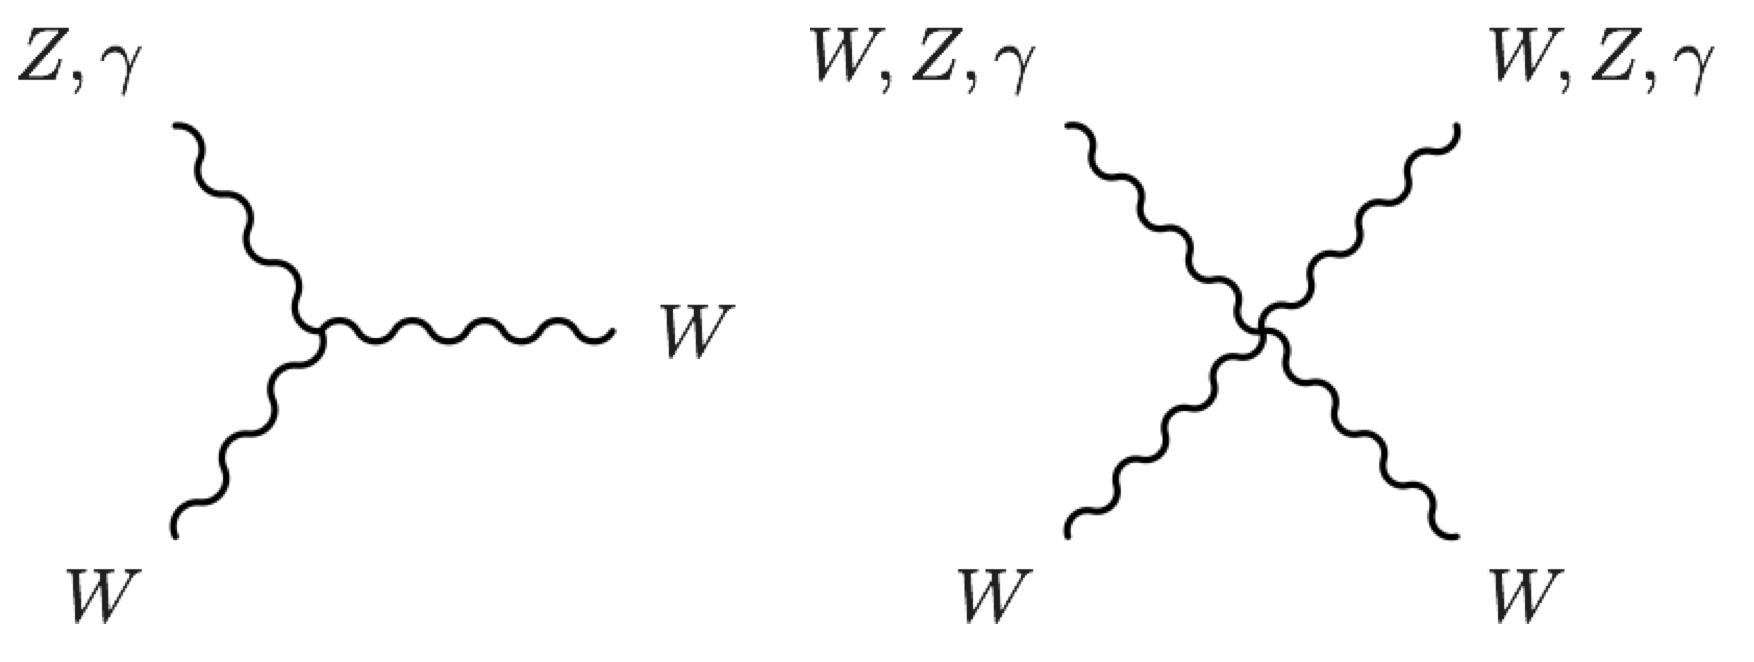
\includegraphics[width=0.65\textwidth]{images/ssWW/vb_self_int.png}
\caption{Feynman diagrams for triple and quartic gauge couplings amongst electroweak gauge bosons. The non-abelian nature of the electroweak force predicts that the gauge bosons can have self-interactions. There are, however, no neutral self-interactions.}
\label{tgcs and qgcs}
\end{figure}

TGCs were extensively studied at the Large Electron-Positron collider \cite{LEP_tgc1,LEP_tgc2,LEP_tgc3,LEP_tgc/qgc2} and the Tevatron \cite{Tevatron_tgc1,Tevatron_tgc2,Tevatron_tgc3} but no evidence was found for QGCs \cite{LEP_tgc/qgc2,LEP_qgc2,LEP_qgc1,Tevatron_qgc2}. The higher energies available at the Large Hadron Collider (LHC) allowed the previously elusive QGCs to be observed \cite{qgc_lhc1,qgc_lhc2,qgc_lhc3}. There are three possible means to investigate QGCs: \textit{tri-boson production}, \textit{exclusive VV production}, and \textit{vector boson scattering} (VBS); see figure \ref{vv_prod}. However tri-boson production has a low cross-section \cite{triboson1,triboson2} and studies of exclusive $VV$ production are complicated by pile-up at hadron colliders \cite{exclusive1,exclusive2}. In contrast VBS has a higher cross-section and distinctive final state VVjj. During the LHC's Run I, the same-sign W-boson scattering cross-section was measured by the ATLAS and CMS collaborations to a significance of 3.6 \cite{ssWW} and 2.0 \cite{ssWW_CMS} standard deviations respectively. More recently, the CMS collaboration published a result using data from the LHC's Run 2, where the cross-section was measured to a significance of 5.5 standard deviations \cite{ssWW_CMS_Run2}.

\begin{figure}
\centering
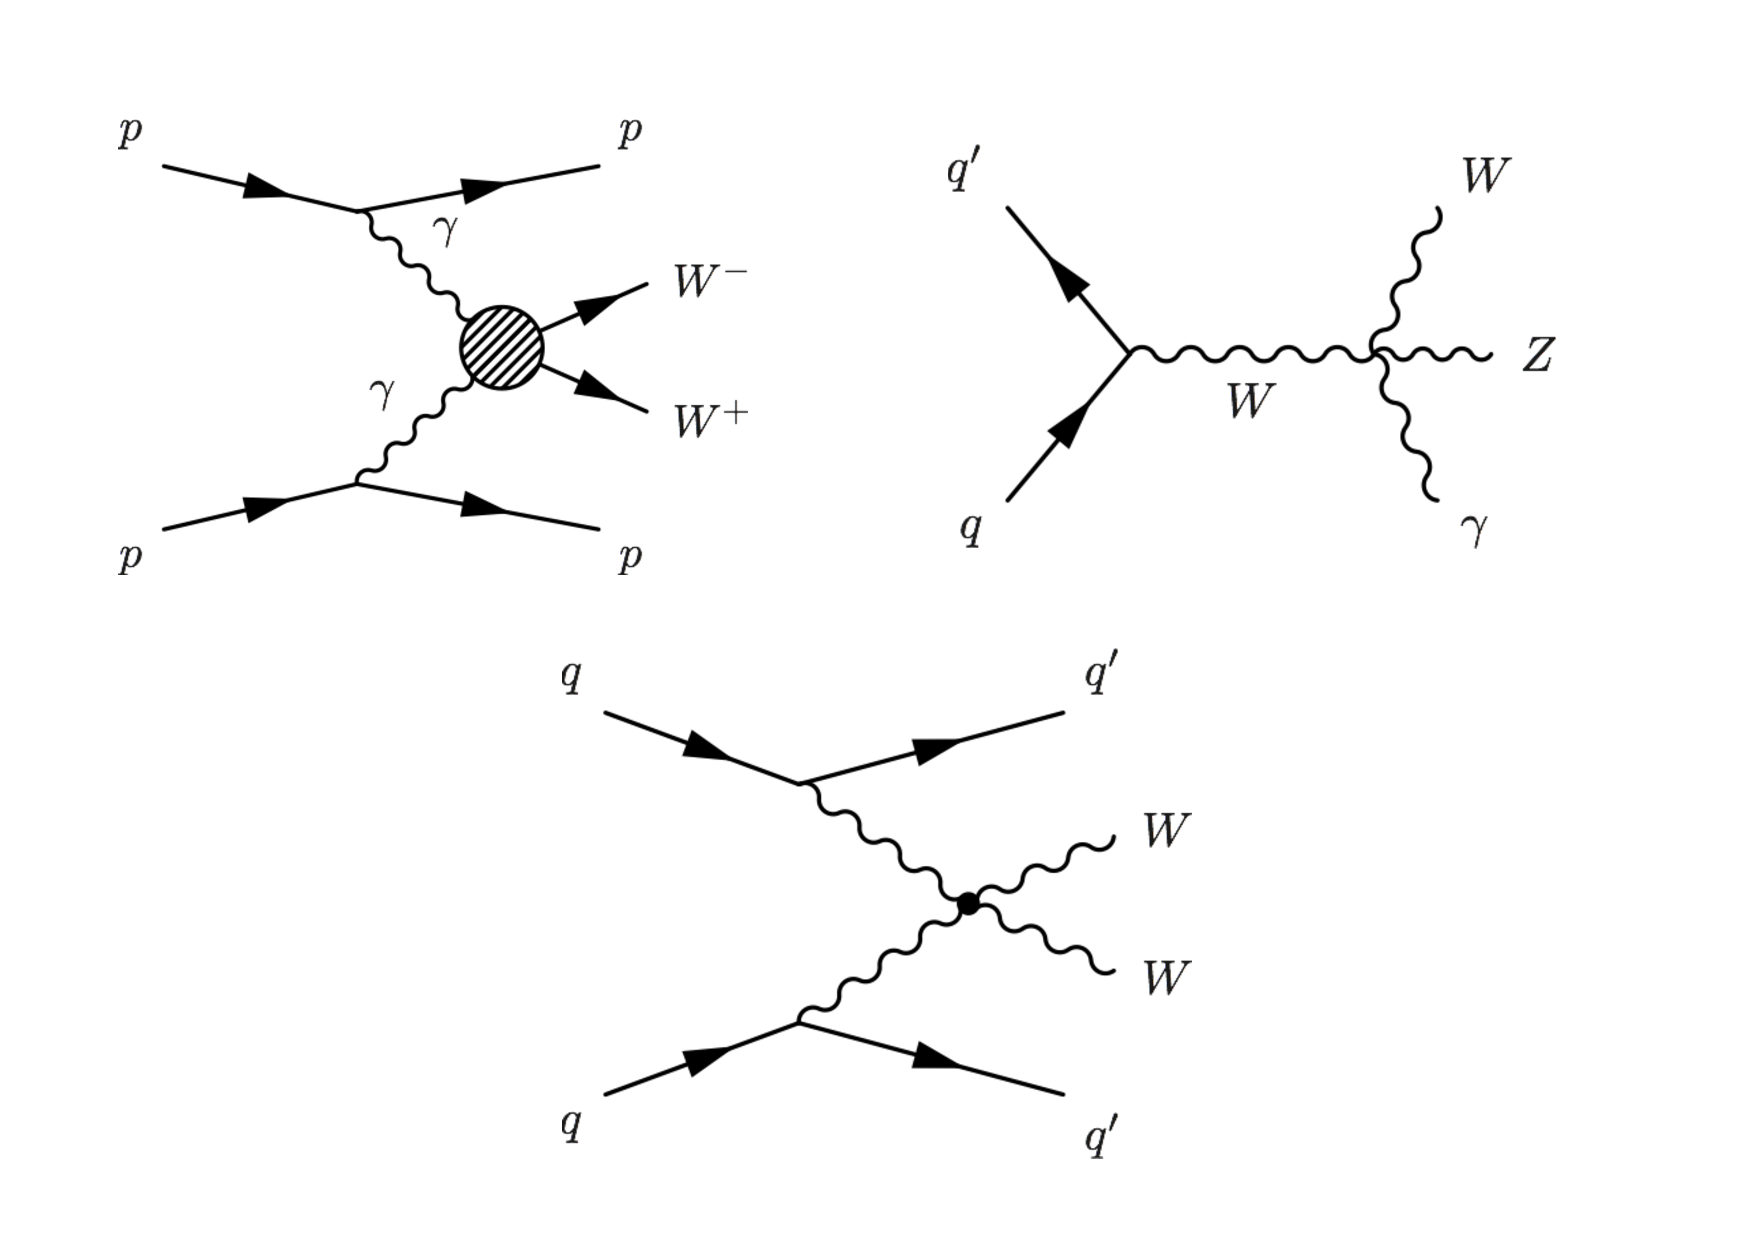
\includegraphics[width=0.85\textwidth]{images/ssWW/VV_prod.pdf}
\caption{Three possible processes for investigating QGCs: at the top on the left, tri-boson production; on the top right, exclusive VV production; and at the bottom, vector boson scattering.}
\label{vv_prod}
\end{figure}

As was discussed in section \ref{Higgs_section}, through the Higgs mechanism, the W and Z-bosons acquire mass which can be interpreted as the longitudinal polarisation component. Without a light SM Higgs-boson, the cross-section for longitudinally polarised VV scattering increases linearly with centre-of-mass energy and violates unitarity at approximately 1 TeV \cite{ssWW} (see figure \ref{x-section_lon_pol_scatt_no_higgs}).

\begin{figure}
\centering
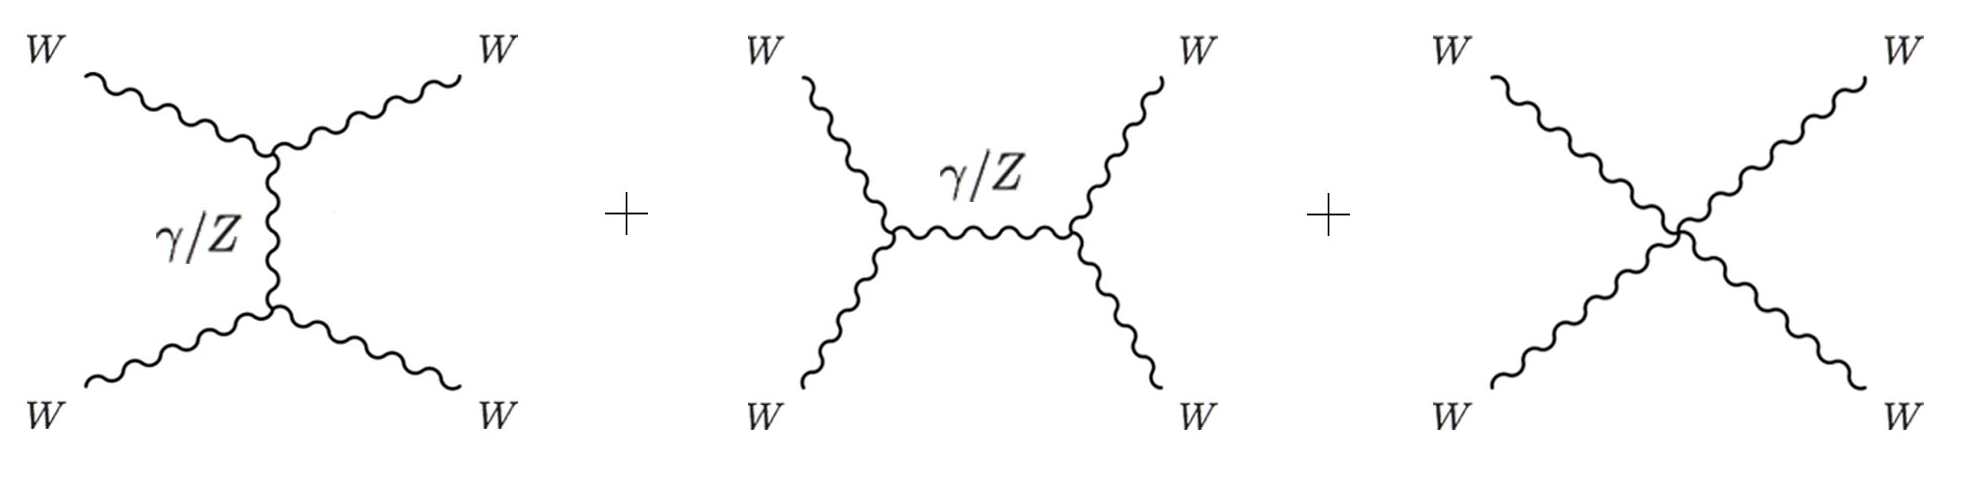
\includegraphics[width=1.\textwidth]{images/ssWW/ww_scatt_diags.png}
\caption{Leading-order Feynman diagrams for $WW \longrightarrow WW$ in the absence of a light SM Higgs-boson.}
\label{ww_scatt_diags}
\end{figure}
\begin{figure}
\centering
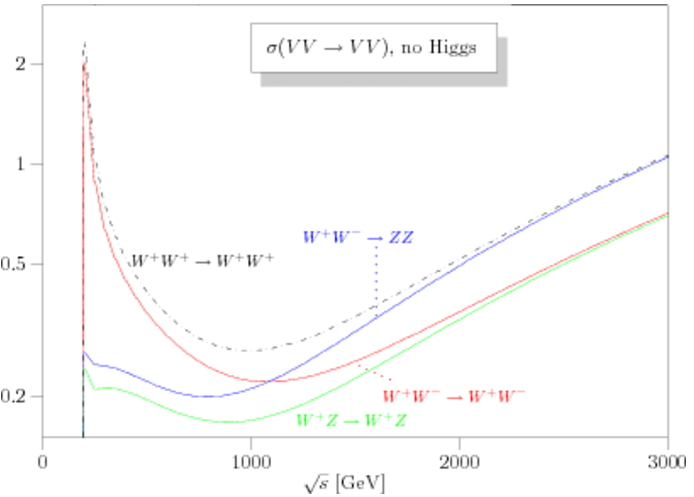
\includegraphics[width=.65\textwidth]{images/ssWW/x-section_lon_pol_scatt_no_higgs.png}
\caption{Longitudinally polarised $VV \longrightarrow VV$ cross-section (in nanobarns) behaviour with $\sqrt{s}$ for four different vector boson scattering processes in the absence of a Higgs-boson. Note that unitarity is violated at approximately 1 TeV. \cite{Alboteanu}}
\label{x-section_lon_pol_scatt_no_higgs}
\end{figure}

However the existence of a light SM Higgs-boson introduces additional diagrams (see figure \ref{new_ww_scatt_diags}), the cross-section becomes regularised \cite{ssWW} (see figure \ref{x-section_lon_pol_scatt_with_higgs}) through the introduction of additional diagrams (compare figures \ref{x-section_lon_pol_scatt_no_higgs} and \ref{x-section_lon_pol_scatt_with_higgs}). This is dealt with in more detail in section \ref{ssWW x-section}.

\begin{figure}
\centering
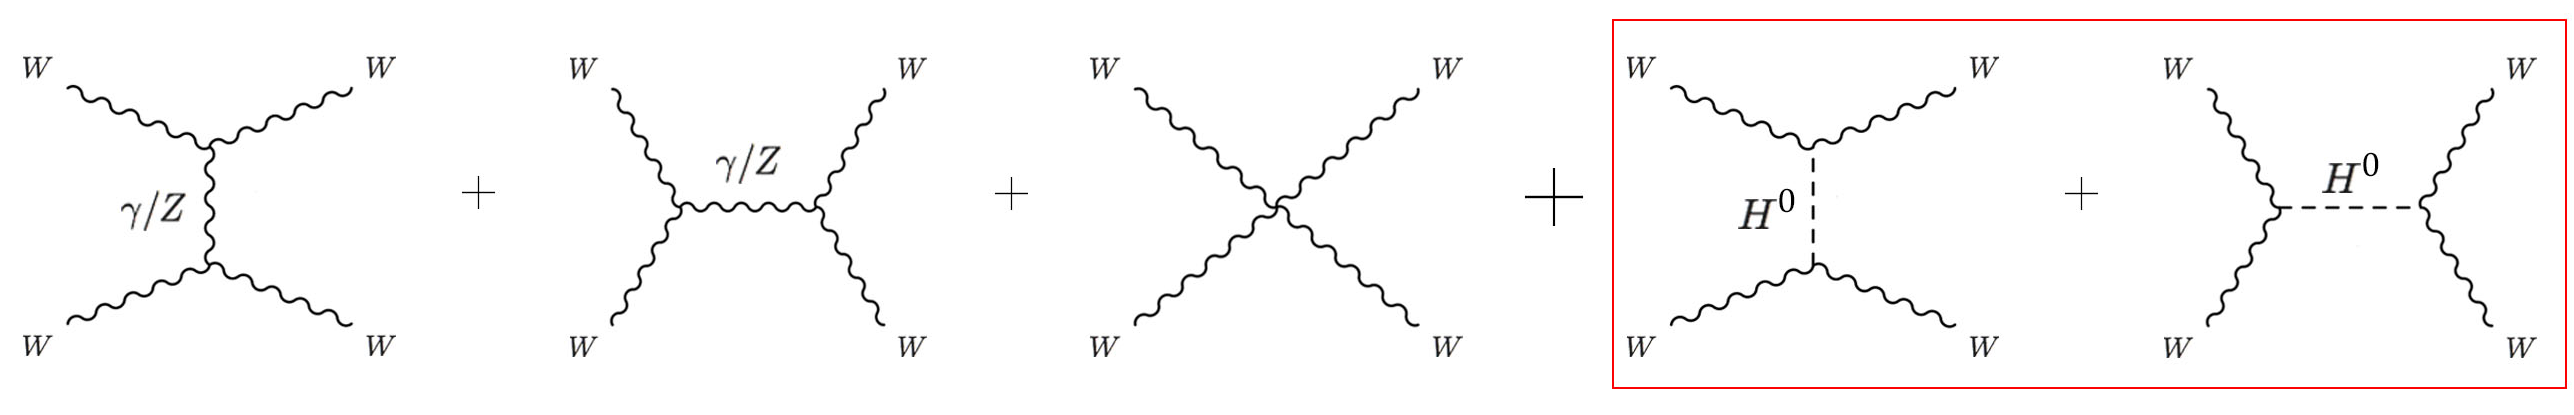
\includegraphics[width=1.\textwidth]{images/ssWW/new_ww_scatt_diags.png}
\caption{Leading-order Feynman diagrams for $WW \longrightarrow WW$ with a light SM Higgs-boson.}
\label{new_ww_scatt_diags}
\end{figure}
\begin{figure}
\centering
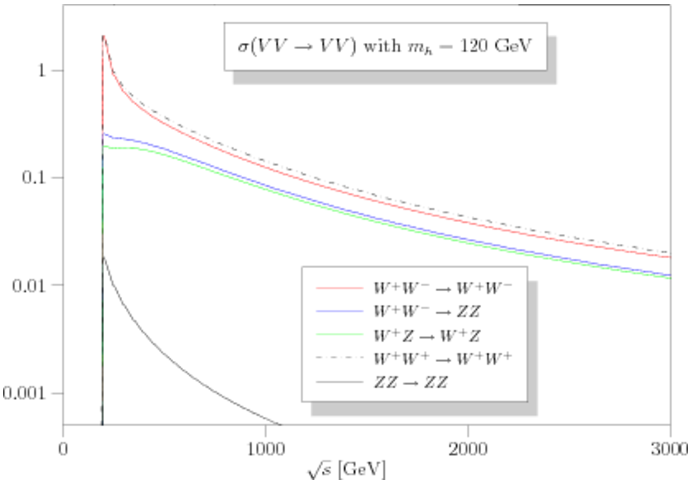
\includegraphics[width=0.65\textwidth]{images/ssWW/x-section_lon_pol_scatt_with_higgs.png}
\caption{Longitudinally polarised $VV \longrightarrow VV$ cross-section behaviour with $\sqrt{s}$ for four different vector boson scattering processes assuming a SM-like Higgs-boson of $120$ GeV mass. The inclusion of the Higgs-boson restores reasonable behaviour of the cross-sections. \cite{Alboteanu}}
\label{x-section_lon_pol_scatt_with_higgs}
\end{figure}

This was a motivation for the existence of a light Higgs-boson prior to its discovery in 2012. At the time of writing this thesis, it is not yet certain whether the 125 GeV Higgs-boson behaves in exactly the way predicted by the SM. VBS could increase understanding of the mechanism of electroweak symmetry breaking. If the vector boson couplings differ from their SM predictions these so-called \emph{anomalous quartic gauge couplings} (aQGCs) may require new physics in order to preserve unitarity, providing additional motivation for studying VBS.

VBS Feynman diagrams are not independently gauge invariant and as a result various non-VBS processes, with the same $VVjj$ final state, must be included in the analysis. These additional non-VBS contributions are classified into electroweak non-VBS production (see figure \ref{ewk_bkg}) and QCD production (see \ref{qcd_bkg}). Certain processes of the non-VBS electroweak production such as VVV or VH production can be gauge invariantly separated and can be suppressed by kinematic cuts. Processes in the QCD production category can be suppressed using topological cuts \cite{ssWW}.

\begin{figure}
\centering
  \centering
  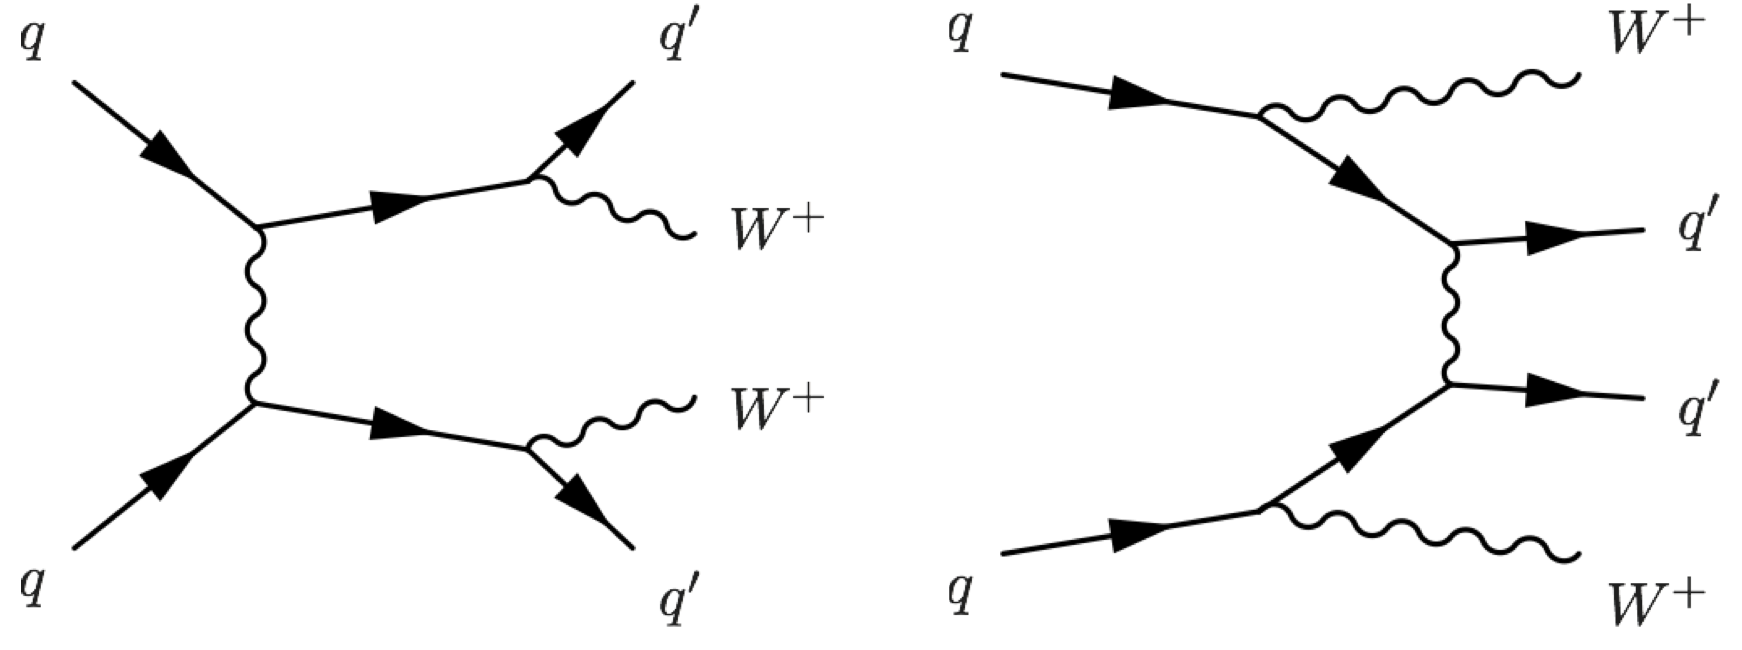
\includegraphics[width=.75\textwidth]{images/ssWW/ewk_bkg.png}
  \caption{Examples of non-VBS electroweak processes with WWjj final state.}
  \label{ewk_bkg}
\end{figure}
\begin{figure}
  \centering
  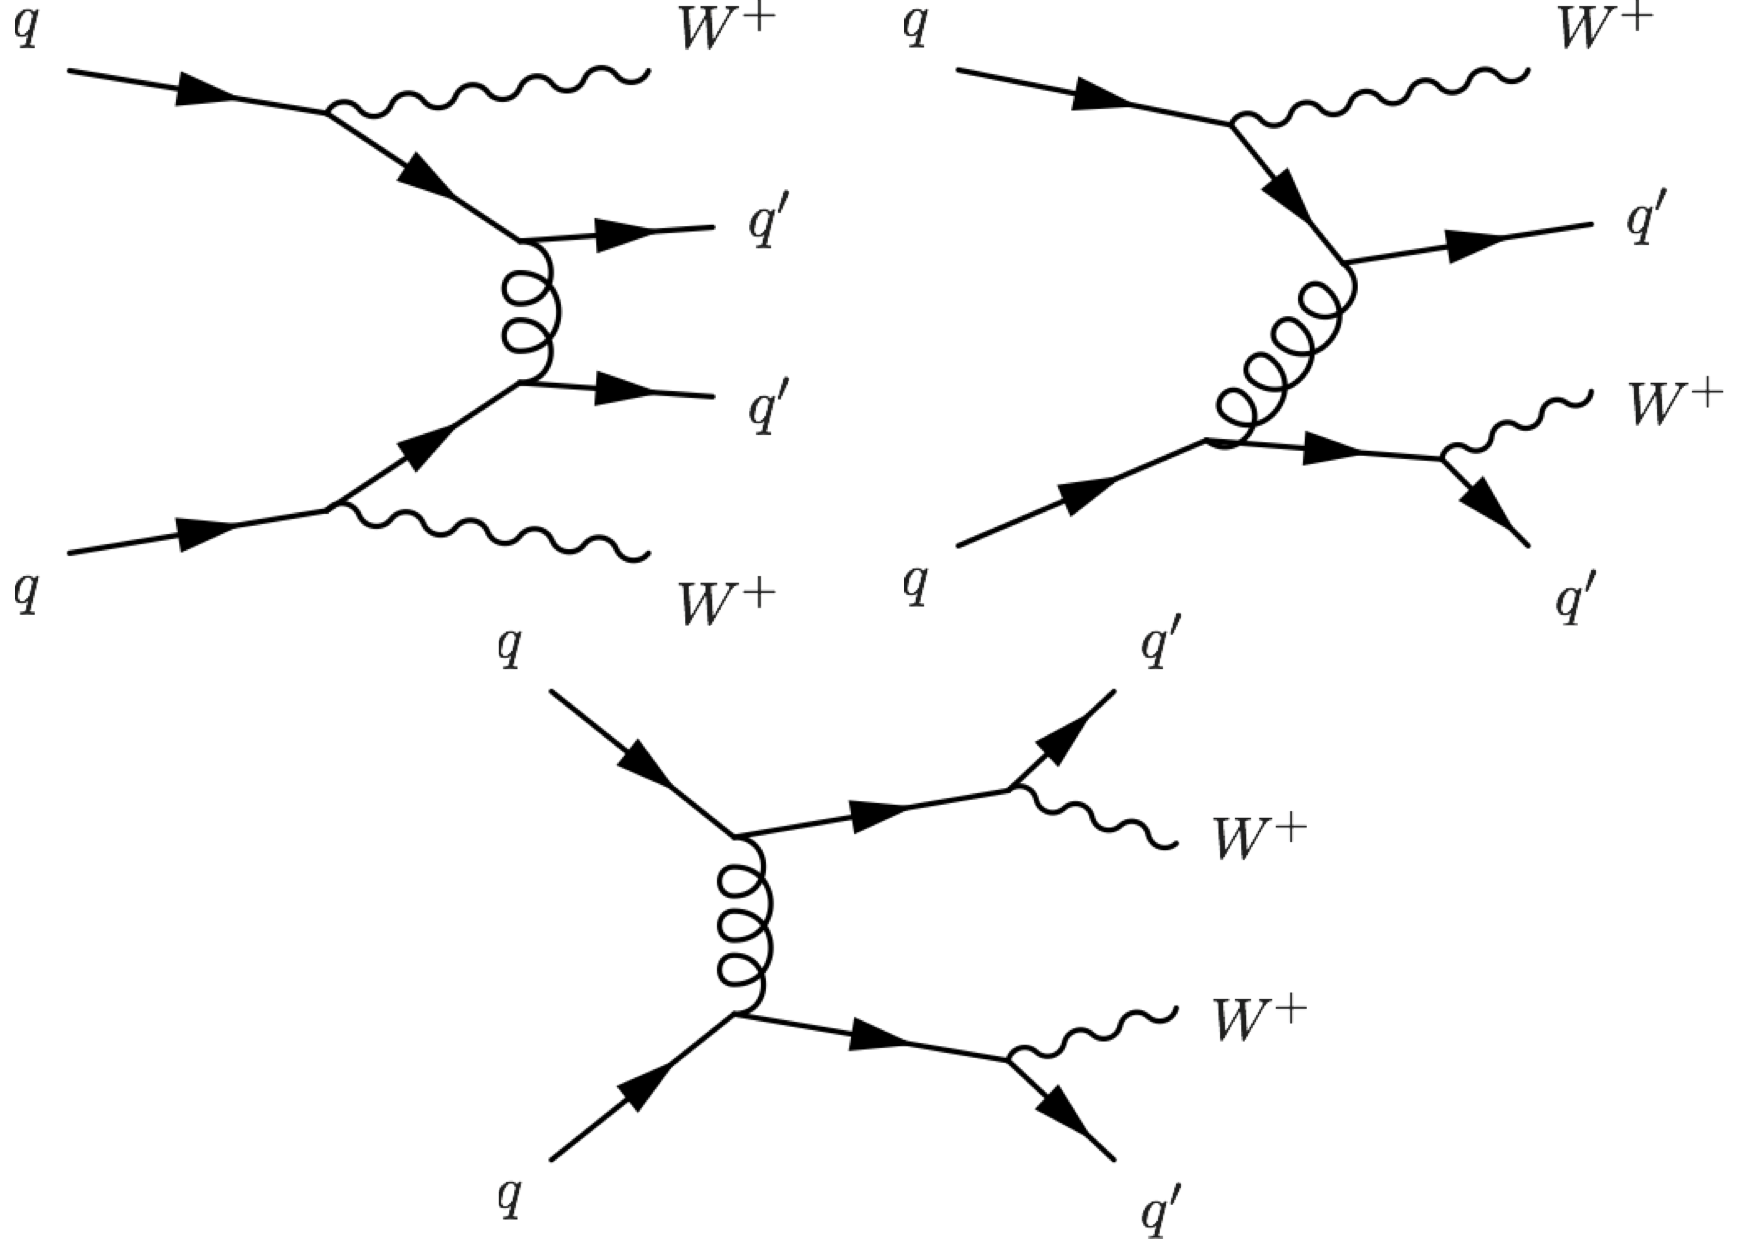
\includegraphics[width=.75\textwidth]{images/ssWW/qcd_bkg.png}
  \caption{Examples of QCD processes with $WWjj$ final state. Can be suppressed by topological cuts.}
  \label{qcd_bkg}
\end{figure}

Vector boson scattering can occur in either the same-sign $W^{\pm}W^{\pm}$ or opposite-sign $W^{\pm}W^{\mp}$ cases. However, the same-sign is preferable for study due to the fact that there is no leading-order gluon-gluon initial state in the same-sign case, in contrast to the opposite-sign case where it does occur (see figure \ref{LO_gluon-gluon}). As a result the $W^{\pm}W^{\pm}jj$ QCD contributions are small when compared to the opposite-sign case (see table \ref{ss_vs_os}). Same-sign W-boson scattering is studied experimentally in the di-lepton channels, considering only electrons ($e$'s) and muons ($\mu$'s), i.e. in the channels $e^{\pm}e^{\pm},e^{\pm}\mu^{\pm},\mu^{\pm}\mu^{\pm}$.\footnote{$\uptau$-leptons are not considered as they are experimentally harder to detect.}

\begin{figure}
\centering
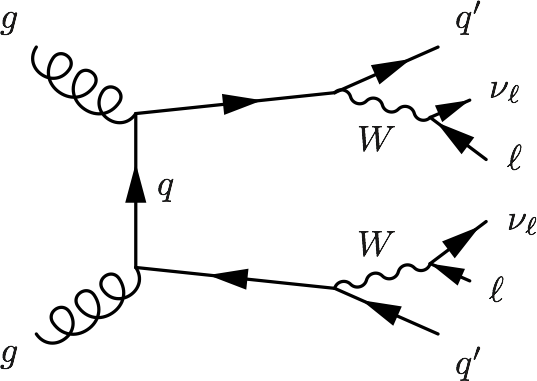
\includegraphics[width=0.4\textwidth]{images/ssWW/LO_gluon-gluon.png}
\caption{Leading-order gluon-gluon $WW$ production. Only possible in the opposite-sign case.}
\label{LO_gluon-gluon}
\end{figure}

\begin{table}
\centering
\begin{tabular}{c c c c}
\hline \hline
Final State & Process & $VVjj$-EW & $VVjj$-QCD \\ \hline 
$\ell^{\pm}\nu\ell^{'\pm}\nu^{'}jj$ (same sign, arbitrary flavour) & $W^{\pm}W^{\pm}$ & $19.5$ fb  & $18.8$ fb \\
$\ell^{\pm}\nu\ell^{'\mp}\nu^{'}jj$ (opposite sign, arbitrary flavour) & $W^{\pm}W^{\mp}$ & $91.3$ fb & $3030$ fb \\
\hline \hline
\end{tabular}
\caption{Comparison of the cross-sections for electroweak and QCD production for both the same-sign and opposite-sign final states at $\sqrt{s}=13$. Note that for the same-sign case the electroweak and QCD cross-sections are the same order of magnitude while this is not true for the opposite sign case. \cite{ssWW}}
\label{ss_vs_os}
\end{table}

Thus same-sign W-boson scattering represents the most promising approach to observe VBS, since the electroweak and QCD contributions are of the same order of magnitude. The distinctive experimental signature is two same-sign leptons, two forward jets, and $E_{T}^{miss}$ carried away by the neutrinos (see figure \ref{ssWW_topology}). Selecting specifically for forward jets helps suppress the QCD background from processes such as quark-quark, or gluon-gluon scattering plus VV radiation, or electroweak VV production plus radiation of gluons resulting in jets. The tagging jets are defined to be the two jets with the highest $p_{T}$ in an event. The tagged jets in $W^{\pm}W^{\pm}jj$ electroweak events tend have a greater difference in rapidity and invariant mass than those in $W^{\pm}W^{\pm}jj$ QCD events. They also tend tend have a larger individual rapidities than their QCD counterparts.

\begin{figure}
\centering
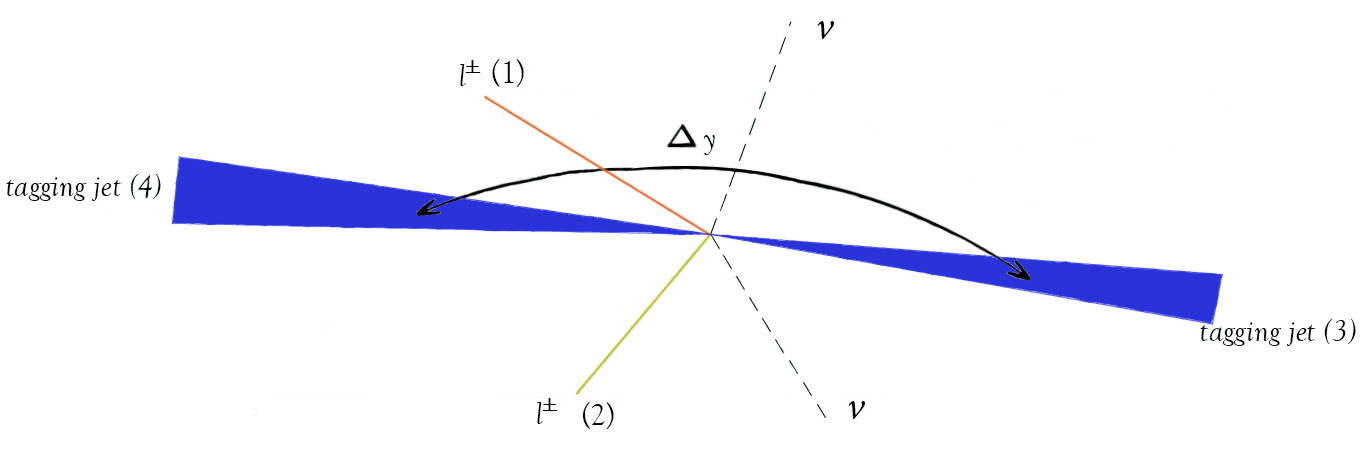
\includegraphics[width=1.0\textwidth]{images/ssWW/ssWW_topology.jpg}
\caption{An illustration of the VBS event topology. Note the charged leptons from the W decay (1,2) and the forward tagging jets (3,4). The invisible neutrinos escape, detectable only through their missing transverse energy. Modified from an image in \cite{ssWW_int_note}.}
\label{ssWW_topology}
\end{figure}

\section{$W^{\pm}W^{\pm}$ Scattering Cross-Section}
\label{ssWW x-section}
Defined initially, in the context of $2\longrightarrow 2$ scattering, are the Lorentz invariant Mandelstam variables:
\begin{eqnarray}
s &=& \left( p - k \right)^{2} = \left( p' + k' \right)^{2} \nonumber \\
t &=& \left(p' - p \right)^{2} = \left(k' - k \right)^{2} \nonumber \\
u &=& \left(k' - p \right)^{2} = \left( p' - k \right)^{2},
\end{eqnarray}
where $p$ and $k$ are the momenta of the initial state particles, and $p'$ and $k'$ are the momenta of the final state particles.

The fact that the electroweak interaction has a non-abelian gauge symmetry means that the gauge bosons are free to scatter off each other. The leading order diagrams for $W^{\pm}W^{\pm}$ scattering that do not involve a Higgs-boson shown in figure \ref{diagrams no higgs}
\begin{figure}
\centering
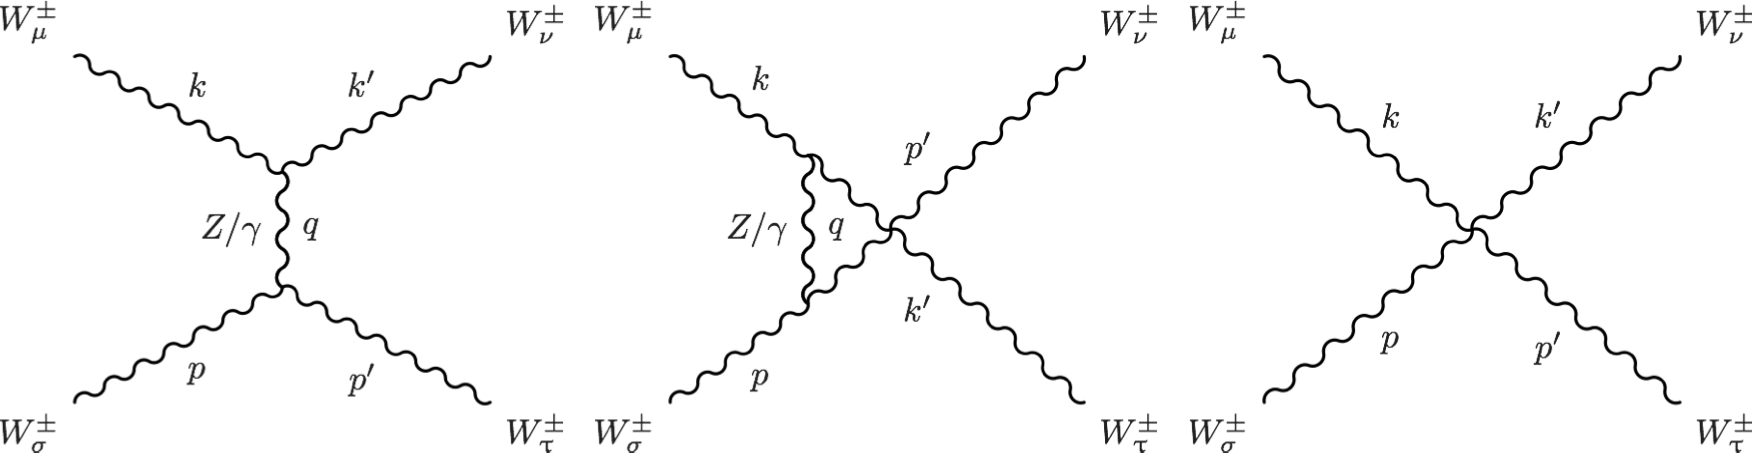
\includegraphics[width=1.0\textwidth]{images/ssWW/diagrams_no_higgs.png}
\caption{Leading-order Feynman diagrams for same-sign W-boson scattering that do not involve a Higgs-boson. Note that the $t$ (left) and $u$ (middle) channel diagrams involve TGCs while the remaining (right) one involves a QGC.}
\label{diagrams no higgs}
\end{figure}

In order to see how the longitudinally polarised scattering amplitude violates unitarity at high energies, apply the Feynman rules for electroweak theory\footnote{See, for example, \cite{mann} or \cite{griffiths}.} to the leading order Feynman diagrams. For the $t$-channel diagram:
\begin{eqnarray}
i \mathcal{M} =& i \hat{\epsilon}_{\mu}(k)\hat{\epsilon}_{\nu}^{*}(k') \left[G^{\mu \nu} \left( k - k' \right)^{\rho} - g^{\mu \rho} \left(q + k \right)^{\nu} + g^{\rho \nu} \left( q + k' \right)^{\mu} \right] \nonumber \\
& \times  \left( \frac{g^{2}c_{W}^{2}}{q^{2} - m_{Z}^{2}} + \frac{g^{2}s_{W}^{2}}{q^{2}} \right)g_{\lambda \rho} \nonumber \\
& \times \left[ g^{\sigma \uptau} \left(p - p' \right)^{\lambda} - g^{\sigma \lambda} \left( q + p \right)^{\uptau} + g^{\lambda \uptau}\left(q +k' \right)^{\sigma} \right] \hat{\epsilon}_{\sigma}(p) \hat{\epsilon}_{\uptau}^{*}(p'),
\end{eqnarray}
for the $u$-channel diagram:
\begin{eqnarray}
i \mathcal{M} = & i \hat{\epsilon}_{\mu}(k) \hat{\epsilon}_{\nu}^{*}(p') \left[ g^{\mu \nu} \left( k - p' \right)^{\rho} - g^{\mu \rho} \left(q + k \right)^{\nu} + g^{\rho \nu} \left( q + p' \right) \right] \nonumber \\
& \times \left( \frac{g^{2}c_{W}^{2}}{q^{2}-m_{Z}^{2}} + \frac{g^{2}s_{W}^{2}}{q^{2}} \right)g_{\lambda \rho} \nonumber \\
&\times \left[ g^{\sigma \uptau} \left(p - k' \right)^{\lambda} - g^{\sigma \lambda} \left( q + p \right)^{\uptau} + g^{\lambda \uptau} \left( q + k' \right)^{\sigma} \right] \hat{\epsilon}_{\sigma}(p)\hat{\epsilon}_{\uptau}^{*}(k'),
\end{eqnarray}
and for the QGC diagram:
\begin{eqnarray}
i \mathcal{M} &= i g^{2} \hat{\epsilon}(k) \hat{\epsilon}_{\nu}^{*}(k')\hat{\epsilon}_{\sigma}(p)\hat{\epsilon}_{\uptau}^{*} \left( 2g^{\mu \nu}g^{\sigma \uptau} - g^{\mu \sigma}g^{\nu \uptau} - g^{\mu \uptau}g^{\nu \sigma} \right),
\end{eqnarray}
where $\hat{\epsilon}$ are the polarisation vectors of the W-bosons, $p$ and $k$ are their momenta, $c_{W}$ and $s_{W}$ are the cosine and sine of the weak mixing angle, which is defined in terms of the weak and hypercharge couplings:
\begin{equation}
s_{W} = \frac{g'}{\sqrt{g^{2} + {g'}^{2}}}.
\end{equation}
The W-bosons considered here are longitudinally polarised. If their four-momentum is given by $k_{\mu} = \left( E_{k},0,0,k \right)$, then the longitudinal polarisation vector is $\hat{\epsilon}_{\mu} = \left( \frac{k}{m},0,0,\frac{E_{k}}{m} \right)$. In the high momentum limit $k >> m$, the polarisation vector can be approximated as:
\begin{eqnarray}
\hat{\epsilon}_{\mu} &=& \left( \frac{k}{m},0,0,\frac{E_{k}}{m} \right) \nonumber \\
&=& \frac{1}{m} \left( E_{k} \sqrt{1-\frac{m^{2}}{E_{k}^{2}}},0,0,k\sqrt{1+\frac{m^{2}}{k^{2}}} \right) \nonumber \\
&\approx& \frac{k^{\mu}}{m}.
\end{eqnarray}
By inserting this approximation in the scattering amplitude, it can be seen that there are terms of $\mathcal{O} \left( \frac{s}{m_{W}^{2}} \right)$ and terms of $\mathcal{O} \left( \frac{s^{2}}{m_{W}^{4}} \right)$. Upon summing the amplitudes, however, the latter terms cancel, leaving $\mathcal{M} \propto \frac{s}{m_{W}^{2}}$.

The cross-section for a $2 \longrightarrow 2$ scattering process with particles of equal mass is given by:
\begin{equation}
\sigma = \frac{1}{32 \pi^{2}s} \int \sqrt{1-\frac{4m^{2}}{s}} \abs{\mathcal{M}}^{2} d\Omega
\end{equation} \cite{griffiths}.
Hence $\sigma \propto \frac{s}{m_{W}^{4}}$, which means the cross-section grows indefinitely with energy and will eventually violate unitarity\footnote{Meaning the probability for the scattering to occur will be greater than 1 (unity), which is unphysical.}. This occurs at approximately 1 TeV.

However if a light Higgs-boson is included then additional diagrams are introduced (see figure \ref{diagrams higgs}). The scattering amplitude for the $t$-channel diagram is:
\begin{equation}
i \mathcal{M} = -ig^{2}m_{W}^{2}\frac{\hat{\epsilon}_{\mu}(k)\hat{\epsilon}_{\nu}^{*}(k')g^{\mu \nu}g^{\sigma \uptau}\hat{\epsilon}_{\sigma}(p)\hat{\epsilon}_{\uptau}^{*}(p')}{q^{2}-m_{h}^{2}},
\end{equation}
and for the $u$-channel:
\begin{equation}
i\mathcal{M} = -ig^{2}m_{W}^{2}\frac{\hat{\epsilon}_{\mu}(k)\hat{\epsilon}_{\nu}^{*}(p')g^{\mu \nu}g^{\sigma \uptau}\hat{\epsilon}_{\sigma}(p)\hat{\epsilon}_{\uptau}^{*}(k')}{q^{2}-m_{h}^{2}}.
\end{equation}
Taking the same limit as before, there are again terms of $\mathcal{O}\left( \frac{s}{m_{W}^{2}} \right)$ but of the opposite sign. These opposite sign contributions cancel exactly with the terms from the previous diagrams such that, in the high energy limit, $\mathcal{M} \propto constant$ instead. The cross-section now decreases with energy and is hence regularised.
\begin{figure}
\centering
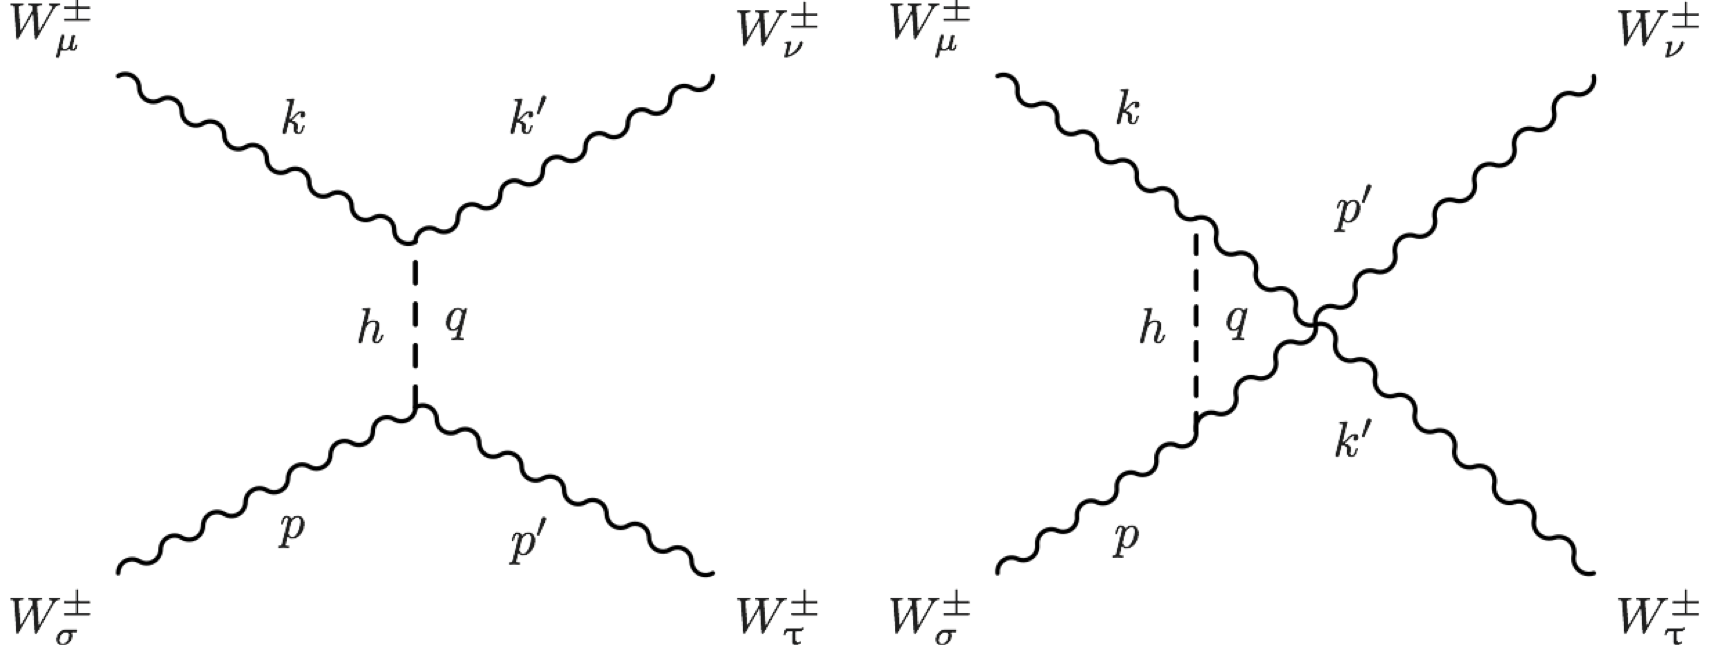
\includegraphics[width=0.75\textwidth]{images/ssWW/diagrams_higgs.png}
\caption{Leading-order Feynman diagrams for same-sign W-boson scattering that involve a Higgs-boson. The $t$-channel diagram is on the left while the $u$-channel diagram is on the right}
\label{diagrams higgs}
\end{figure}